\subsubsection{Simulation of the Controllers}
The simulations show the behavior of the $z_{\mathrm{I}}$ velocity and position controllers when subjected to a step input reference signal and acting on the non-linear plant.

In \autoref{fig:velocityControllerZ}, a step reference of \SI{1}{m s^{-1}} is given to the controller. This reveals a rise time of approximately \SI{0.4}{s}, an overshoot of 16.4 percent and a settling time of \SI{2.5}{s}.

The control action required by the $z_{\mathrm{I}}$ velocity controller is shown in \autoref{fig:velocityControllerZAction}. This is the sum of rotational speeds in the motors, which is added to the equilibrium speeds to achieve the response in \autoref{fig:velocityControllerZ}.

\begin{minipage}{\linewidth}
    \begin{minipage}{0.45\linewidth}
        \begin{figure}[H]
            \vspace{-.4cm}
            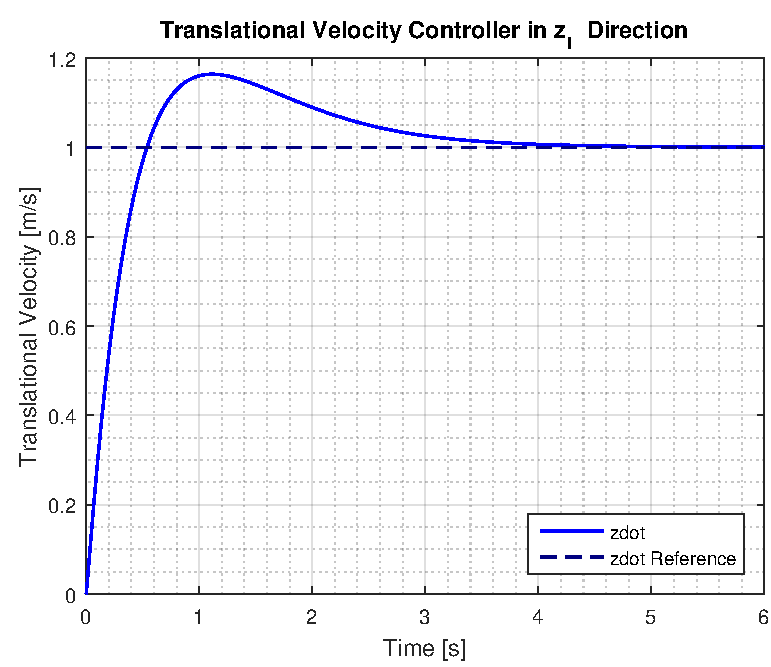
\includegraphics[scale=.5]{figures/velocityControllerZ}
            \centering			
            \captionof{figure}{Step response of the $z_{\mathrm{I}}$ velocity controller.}
            \label{fig:velocityControllerZ}
        \end{figure}
    \end{minipage}
    \hspace{0.03\linewidth}
    \begin{minipage}{0.45\linewidth}
        \begin{figure}[H]
            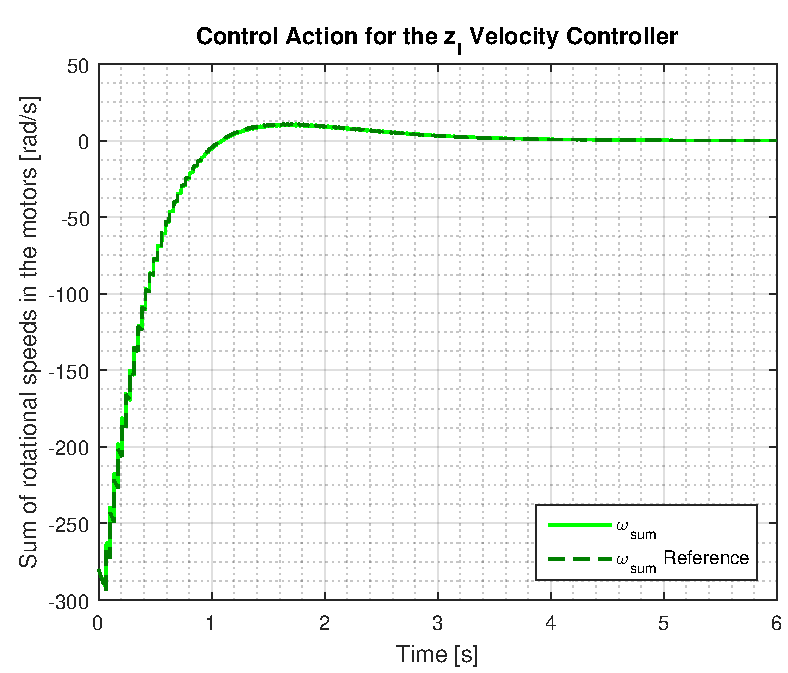
\includegraphics[scale=.5]{figures/velocityControllerZAction}
            \centering
            \captionof{figure}{Control action required by the $z_{\mathrm{I}}$ velocity controller to achieve the response in \autoref{fig:velocityControllerZ}.}
            \label{fig:velocityControllerZAction}
        \end{figure}
    \end{minipage}
\end{minipage}

The $z_{\mathrm{I}}$ position controller response is seen in \autoref{fig:positionControllersZ}. A step reference of \SI{1}{m} is imposed on the controller. This reveals a rise time of \SI{1.25}{s} and a settling time of \SI{1.8}{s}. In \autoref{fig:positionControllerZAction}, the control action imposed by the position controller is shown. This is the translational velocity, which is denoted "zdot Reference" in \autoref{fig:positionControllerZAction}. "zdot" is the velocity applied by the velocity controller.
\begin{minipage}{\linewidth}
    \begin{minipage}{0.45\linewidth}
        \begin{figure}[H]
            \vspace{-1.3cm}
            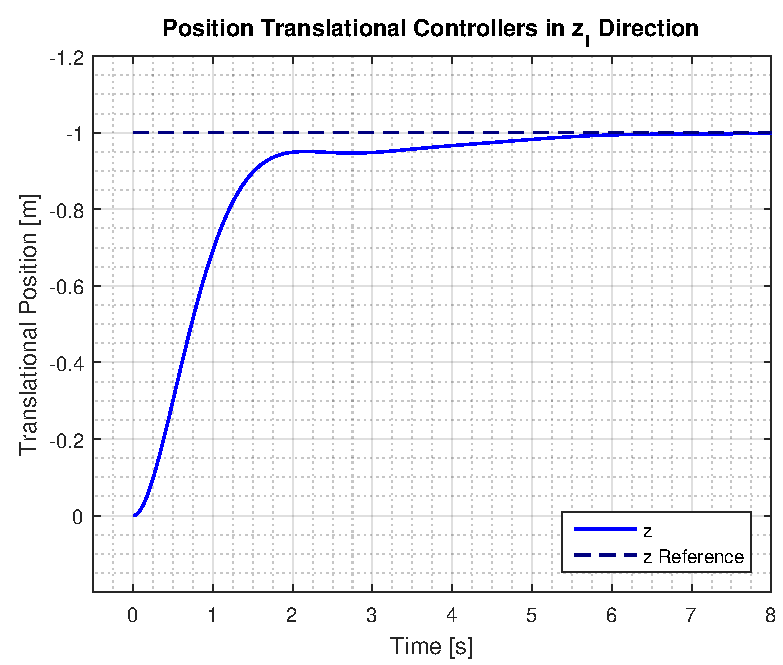
\includegraphics[scale=.55]{figures/positionControllerZ}
            \centering			
            \captionof{figure}{Step response of the $z_{\mathrm{I}}$ position controller.}
            \label{fig:positionControllersZ}
        \end{figure}
    \end{minipage}
    \hspace{0.03\linewidth}
    \begin{minipage}{0.45\linewidth}
        \begin{figure}[H]
            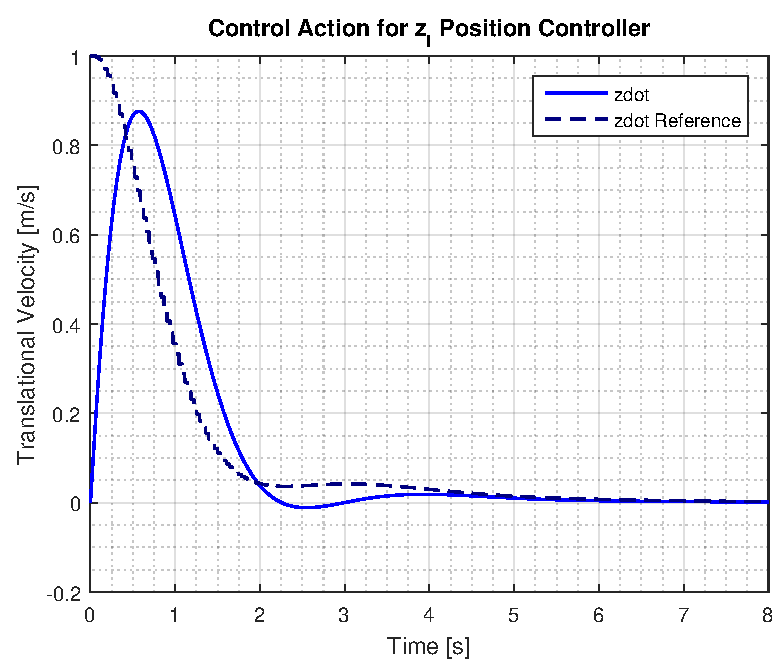
\includegraphics[scale=.55]{figures/positionControllerZAction}
            \centering
            \captionof{figure}{Control action imposed by the $z_{\mathrm{I}}$ position controller to track the step reference and the performance of the inner velocity controller seen in \autoref{fig:positionControllersZ}.}
            \label{fig:positionControllerZAction}
        \end{figure}
    \end{minipage}
\end{minipage}